
% This LaTeX was auto-generated from MATLAB code.
% To make changes, update the MATLAB code and republish this document.

\documentclass{article}
\usepackage{graphicx}
\usepackage{color}

\sloppy
\definecolor{lightgray}{gray}{0.5}
\setlength{\parindent}{0pt}

\begin{document}

    
    \begin{verbatim}
function thirdTask
% Задаване на параметри
a = 1; b = 4; % граници на интервала
alpha = -0.3; %x(a)=alpha
beta = 0.4; % x(b)=beta
n = 150; % брой точки на дискретизация
h = (b-a)/(n+1); % стъпка на дискретизация

% Дефиниране на матрицата на коефициентите и вектора на дясната страна
A = zeros(n,n);
f = zeros(n,1);
for i = 1:n
    ti = a + i*h;
    A(i,i) = -2/h^2 + 16/ti^2;
    f(i) = h^2*sin(1/ti^2);
    if i ~= 1
        A(i,i-1) = 1/h^2 - 1/(2*h*ti);
    end
    if i ~= n
        A(i,i+1) = 1/h^2 + 1/(2*h*ti);
    end
end

% Прилагане на граничните условия
A(1,:) = 0; A(1,1) = 1;
f(1) = alpha;
A(n,:) = 0; A(n,n) = 1;
f(n) = beta;

% Решаване на системата
x = A\f;

% Визуализация на решението
t = linspace(a,b,n+2);
xx=[alpha;x;beta];
figure(3),plot(t,xx);
xlabel('t');
ylabel('x(t)');
title('Решение по метода на крайните приближения');
end
\end{verbatim}

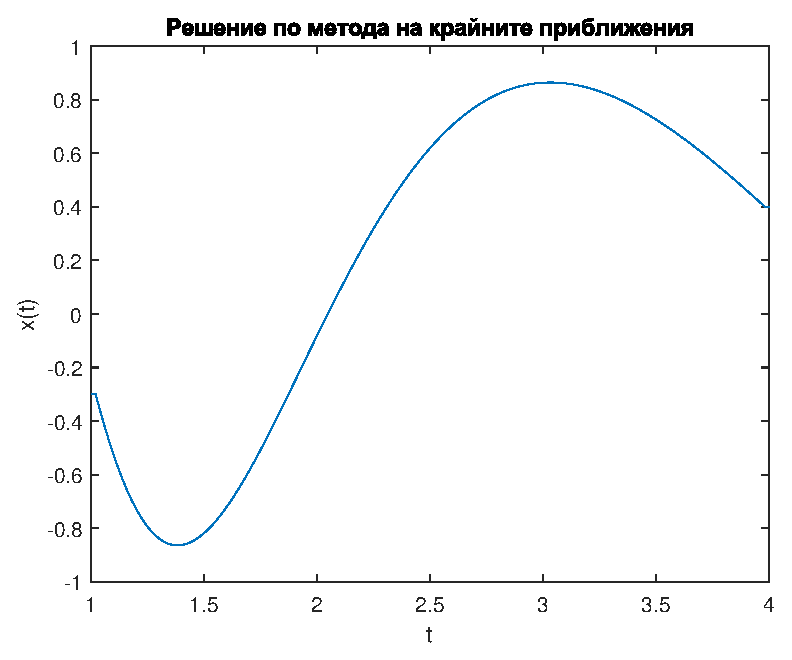
\includegraphics [width=4in]{thirdTask_01.eps}



\end{document}

